\documentclass[1p]{elsarticle_modified}
%\bibliographystyle{elsarticle-num}

%\usepackage[colorlinks]{hyperref}
%\usepackage{abbrmath_seonhwa} %\Abb, \Ascr, \Acal ,\Abf, \Afrak
\usepackage{amsfonts}
\usepackage{amssymb}
\usepackage{amsmath}
\usepackage{amsthm}
\usepackage{scalefnt}
\usepackage{amsbsy}
\usepackage{kotex}
\usepackage{caption}
\usepackage{subfig}
\usepackage{color}
\usepackage{graphicx}
\usepackage{xcolor} %% white, black, red, green, blue, cyan, magenta, yellow
\usepackage{float}
\usepackage{setspace}
\usepackage{hyperref}

\usepackage{tikz}
\usetikzlibrary{arrows}

\usepackage{multirow}
\usepackage{array} % fixed length table
\usepackage{hhline}

%%%%%%%%%%%%%%%%%%%%%
\makeatletter
\renewcommand*\env@matrix[1][\arraystretch]{%
	\edef\arraystretch{#1}%
	\hskip -\arraycolsep
	\let\@ifnextchar\new@ifnextchar
	\array{*\c@MaxMatrixCols c}}
\makeatother %https://tex.stackexchange.com/questions/14071/how-can-i-increase-the-line-spacing-in-a-matrix
%%%%%%%%%%%%%%%

\usepackage[normalem]{ulem}

\newcommand{\msout}[1]{\ifmmode\text{\sout{\ensuremath{#1}}}\else\sout{#1}\fi}
%SOURCE: \msout is \stkout macro in https://tex.stackexchange.com/questions/20609/strikeout-in-math-mode

\newcommand{\cancel}[1]{
	\ifmmode
	{\color{red}\msout{#1}}
	\else
	{\color{red}\sout{#1}}
	\fi
}

\newcommand{\add}[1]{
	{\color{blue}\uwave{#1}}
}

\newcommand{\replace}[2]{
	\ifmmode
	{\color{red}\msout{#1}}{\color{blue}\uwave{#2}}
	\else
	{\color{red}\sout{#1}}{\color{blue}\uwave{#2}}
	\fi
}

\newcommand{\Sol}{\mathcal{S}} %segment
\newcommand{\D}{D} %diagram
\newcommand{\A}{\mathcal{A}} %arc


%%%%%%%%%%%%%%%%%%%%%%%%%%%%%5 test

\def\sl{\operatorname{\textup{SL}}(2,\Cbb)}
\def\psl{\operatorname{\textup{PSL}}(2,\Cbb)}
\def\quan{\mkern 1mu \triangleright \mkern 1mu}

\theoremstyle{definition}
\newtheorem{thm}{Theorem}[section]
\newtheorem{prop}[thm]{Proposition}
\newtheorem{lem}[thm]{Lemma}
\newtheorem{ques}[thm]{Question}
\newtheorem{cor}[thm]{Corollary}
\newtheorem{defn}[thm]{Definition}
\newtheorem{exam}[thm]{Example}
\newtheorem{rmk}[thm]{Remark}
\newtheorem{alg}[thm]{Algorithm}

\newcommand{\I}{\sqrt{-1}}
\begin{document}

%\begin{frontmatter}
%
%\title{Boundary parabolic representations of knots up to 8 crossings}
%
%%% Group authors per affiliation:
%\author{Yunhi Cho} 
%\address{Department of Mathematics, University of Seoul, Seoul, Korea}
%\ead{yhcho@uos.ac.kr}
%
%
%\author{Seonhwa Kim} %\fnref{s_kim}}
%\address{Center for Geometry and Physics, Institute for Basic Science, Pohang, 37673, Korea}
%\ead{ryeona17@ibs.re.kr}
%
%\author{Hyuk Kim}
%\address{Department of Mathematical Sciences, Seoul National University, Seoul 08826, Korea}
%\ead{hyukkim@snu.ac.kr}
%
%\author{Seokbeom Yoon}
%\address{Department of Mathematical Sciences, Seoul National University, Seoul, 08826,  Korea}
%\ead{sbyoon15@snu.ac.kr}
%
%\begin{abstract}
%We find all boundary parabolic representation of knots up to 8 crossings.
%
%\end{abstract}
%\begin{keyword}
%    \MSC[2010] 57M25 
%\end{keyword}
%
%\end{frontmatter}

%\linenumbers
%\tableofcontents
%
\newcommand\colored[1]{\textcolor{white}{\rule[-0.35ex]{0.8em}{1.4ex}}\kern-0.8em\color{red} #1}%
%\newcommand\colored[1]{\textcolor{white}{ #1}\kern-2.17ex	\textcolor{white}{ #1}\kern-1.81ex	\textcolor{white}{ #1}\kern-2.15ex\color{red}#1	}

{\Large $\underline{11a_{131}~(K11a_{131})}$}

\setlength{\tabcolsep}{10pt}
\renewcommand{\arraystretch}{1.6}
\vspace{1cm}\begin{tabular}{m{100pt}>{\centering\arraybackslash}m{274pt}}
\multirow{5}{120pt}{
	\centering
	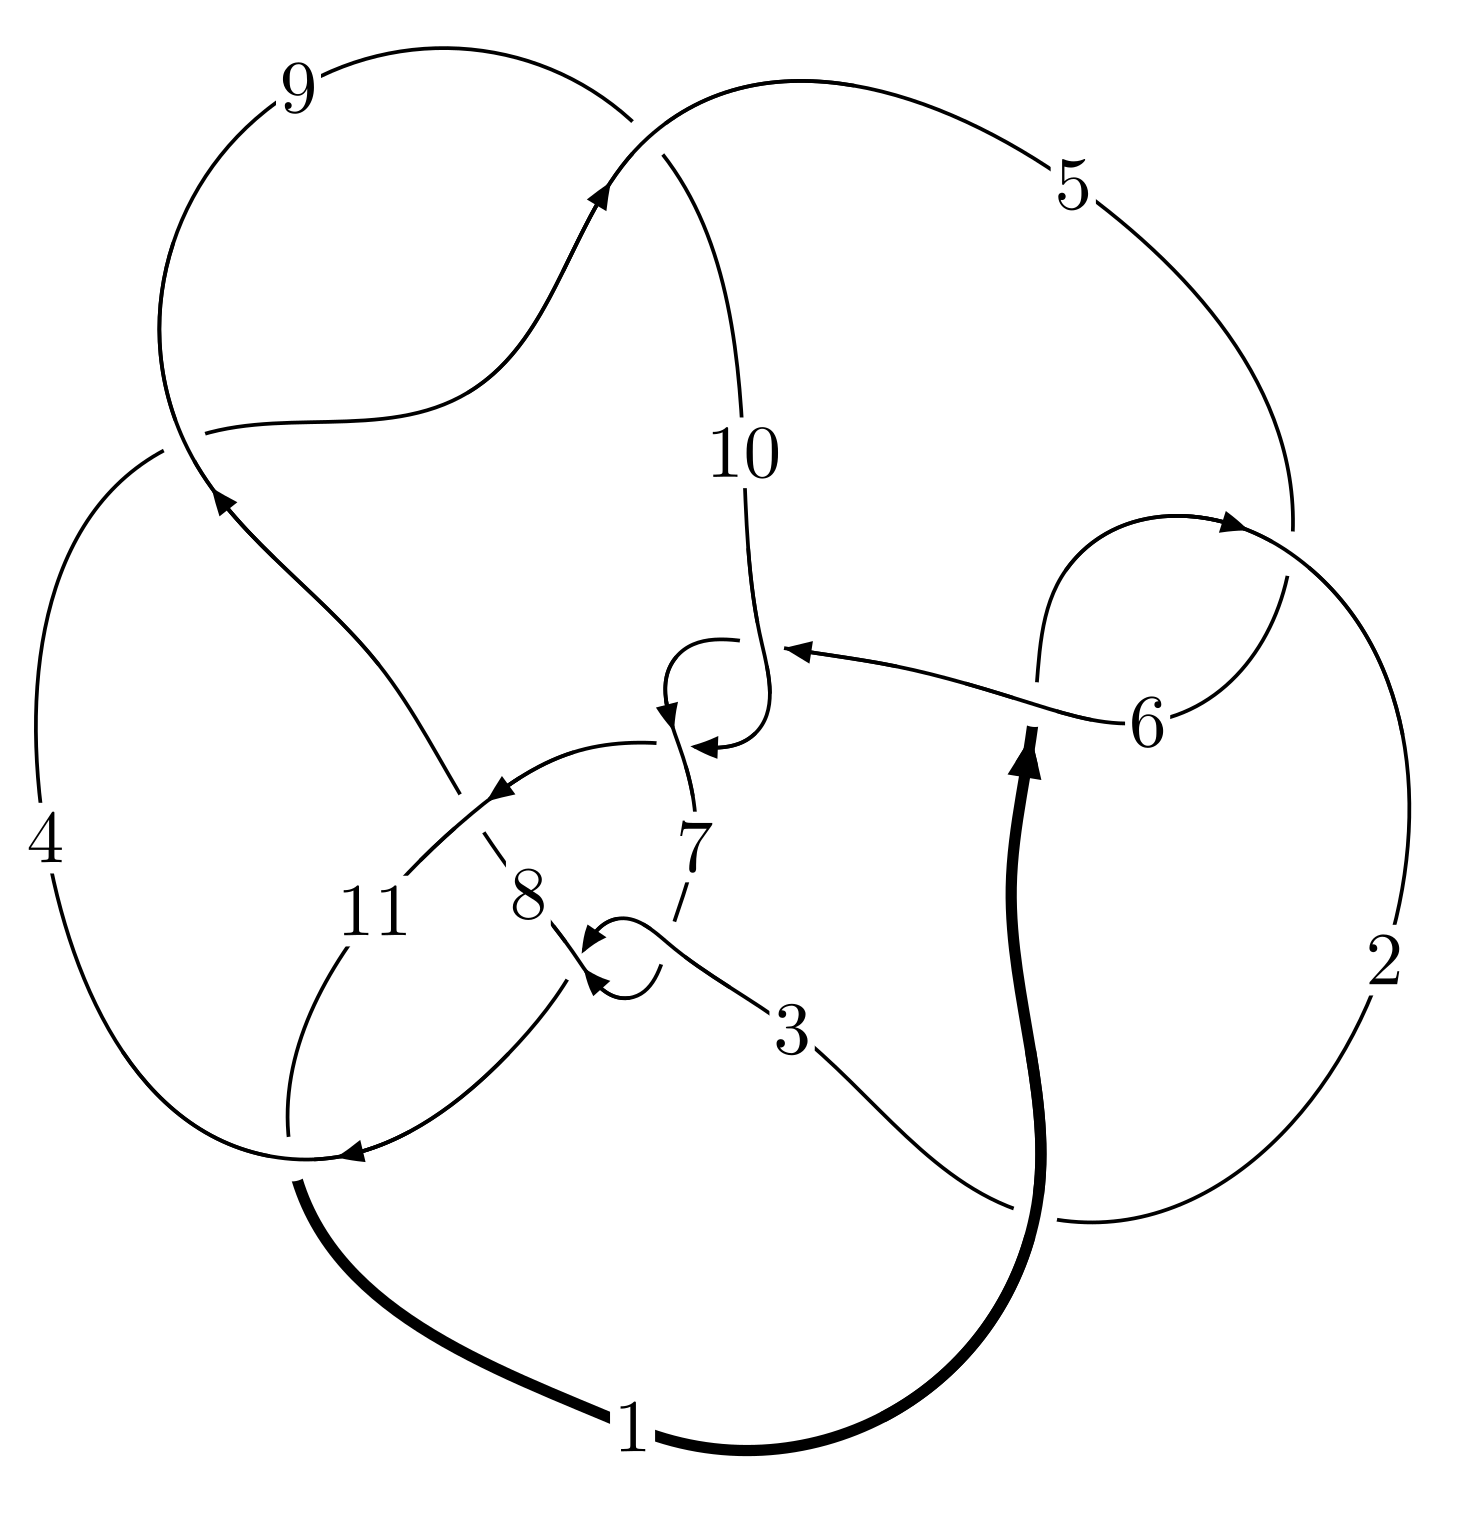
\includegraphics[width=112pt]{../../../GIT/diagram.site/Diagrams/png/380_11a_131.png}\\
\ \ \ A knot diagram\footnotemark}&
\allowdisplaybreaks
\textbf{Linearized knot diagam} \\
\cline{2-2}
 &
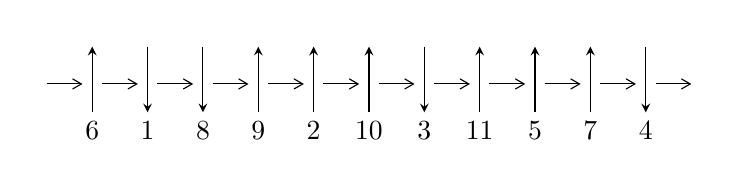
\begin{tikzpicture}[x=20pt, y=17pt]
	% nodes
	\node (C0) at (0, 0) {};
	\node (C1) at (1, 0) {};
	\node (C1U) at (1, +1) {};
	\node (C1D) at (1, -1) {6};

	\node (C2) at (2, 0) {};
	\node (C2U) at (2, +1) {};
	\node (C2D) at (2, -1) {1};

	\node (C3) at (3, 0) {};
	\node (C3U) at (3, +1) {};
	\node (C3D) at (3, -1) {8};

	\node (C4) at (4, 0) {};
	\node (C4U) at (4, +1) {};
	\node (C4D) at (4, -1) {9};

	\node (C5) at (5, 0) {};
	\node (C5U) at (5, +1) {};
	\node (C5D) at (5, -1) {2};

	\node (C6) at (6, 0) {};
	\node (C6U) at (6, +1) {};
	\node (C6D) at (6, -1) {10};

	\node (C7) at (7, 0) {};
	\node (C7U) at (7, +1) {};
	\node (C7D) at (7, -1) {3};

	\node (C8) at (8, 0) {};
	\node (C8U) at (8, +1) {};
	\node (C8D) at (8, -1) {11};

	\node (C9) at (9, 0) {};
	\node (C9U) at (9, +1) {};
	\node (C9D) at (9, -1) {5};

	\node (C10) at (10, 0) {};
	\node (C10U) at (10, +1) {};
	\node (C10D) at (10, -1) {7};

	\node (C11) at (11, 0) {};
	\node (C11U) at (11, +1) {};
	\node (C11D) at (11, -1) {4};
	\node (C12) at (12, 0) {};

	% arrows
	\draw[->,>={angle 60}]
	(C0) edge (C1) (C1) edge (C2) (C2) edge (C3) (C3) edge (C4) (C4) edge (C5) (C5) edge (C6) (C6) edge (C7) (C7) edge (C8) (C8) edge (C9) (C9) edge (C10) (C10) edge (C11) (C11) edge (C12) ;	\draw[->,>=stealth]
	(C1D) edge (C1U) (C2U) edge (C2D) (C3U) edge (C3D) (C4D) edge (C4U) (C5D) edge (C5U) (C6D) edge (C6U) (C7U) edge (C7D) (C8D) edge (C8U) (C9D) edge (C9U) (C10D) edge (C10U) (C11U) edge (C11D) ;
	\end{tikzpicture} \\
\hhline{~~} \\& 
\textbf{Solving Sequence} \\ \cline{2-2} 
 &
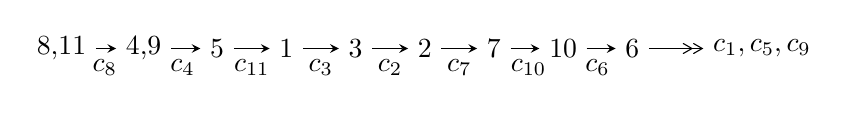
\begin{tikzpicture}[x=25pt, y=7pt]
	% node
	\node (A0) at (-1/8, 0) {8,11};
	\node (A1) at (17/16, 0) {4,9};
	\node (A2) at (17/8, 0) {5};
	\node (A3) at (25/8, 0) {1};
	\node (A4) at (33/8, 0) {3};
	\node (A5) at (41/8, 0) {2};
	\node (A6) at (49/8, 0) {7};
	\node (A7) at (57/8, 0) {10};
	\node (A8) at (65/8, 0) {6};
	\node (C1) at (1/2, -1) {$c_{8}$};
	\node (C2) at (13/8, -1) {$c_{4}$};
	\node (C3) at (21/8, -1) {$c_{11}$};
	\node (C4) at (29/8, -1) {$c_{3}$};
	\node (C5) at (37/8, -1) {$c_{2}$};
	\node (C6) at (45/8, -1) {$c_{7}$};
	\node (C7) at (53/8, -1) {$c_{10}$};
	\node (C8) at (61/8, -1) {$c_{6}$};
	\node (A9) at (10, 0) {$c_{1},c_{5},c_{9}$};

	% edge
	\draw[->,>=stealth]	
	(A0) edge (A1) (A1) edge (A2) (A2) edge (A3) (A3) edge (A4) (A4) edge (A5) (A5) edge (A6) (A6) edge (A7) (A7) edge (A8) ;
	\draw[->>,>={angle 60}]	
	(A8) edge (A9);
\end{tikzpicture} \\ 

\end{tabular} \\

\footnotetext{
The image of knot diagram is generated by the software ``\textbf{Draw programme}" developed by Andrew Bartholomew(\url{http://www.layer8.co.uk/maths/draw/index.htm\#Running-draw}), where we modified some parts for our purpose(\url{https://github.com/CATsTAILs/LinksPainter}).
}\phantom \\ \newline 
\centering \textbf{Ideals for irreducible components\footnotemark of $X_{\text{par}}$} 
 
\begin{align*}
I^u_{1}&=\langle 
-2.39241\times10^{297} u^{76}+2.07034\times10^{298} u^{75}+\cdots+7.56609\times10^{293} b-6.88514\times10^{297},\\
\phantom{I^u_{1}}&\phantom{= \langle  }1.90621\times10^{298} u^{76}-1.65962\times10^{299} u^{75}+\cdots+7.56609\times10^{293} a+6.40142\times10^{298},\;u^{77}-9 u^{76}+\cdots+21 u-1\rangle \\
I^u_{2}&=\langle 
265 u^{11}+395 u^{10}+\cdots+b+529,\\
\phantom{I^u_{2}}&\phantom{= \langle  }62 u^{11}+109 u^{10}+31 u^9-12 u^8+252 u^7-61 u^6-934 u^5-809 u^4+808 u^3+1745 u^2+a+992 u+184,\\
\phantom{I^u_{2}}&\phantom{= \langle  }u^{12}+2 u^{11}+u^{10}+4 u^8-15 u^6-17 u^5+9 u^4+31 u^3+24 u^2+8 u+1\rangle \\
\\
\end{align*}
\raggedright * 2 irreducible components of $\dim_{\mathbb{C}}=0$, with total 89 representations.\\
\footnotetext{All coefficients of polynomials are rational numbers. But the coefficients are sometimes approximated in decimal forms when there is not enough margin.}
\newpage
\renewcommand{\arraystretch}{1}
\centering \section*{I. $I^u_{1}= \langle -2.39\times10^{297} u^{76}+2.07\times10^{298} u^{75}+\cdots+7.57\times10^{293} b-6.89\times10^{297},\;1.91\times10^{298} u^{76}-1.66\times10^{299} u^{75}+\cdots+7.57\times10^{293} a+6.40\times10^{298},\;u^{77}-9 u^{76}+\cdots+21 u-1 \rangle$}
\flushleft \textbf{(i) Arc colorings}\\
\begin{tabular}{m{7pt} m{180pt} m{7pt} m{180pt} }
\flushright $a_{8}=$&$\begin{pmatrix}1\\0\end{pmatrix}$ \\
\flushright $a_{11}=$&$\begin{pmatrix}0\\u\end{pmatrix}$ \\
\flushright $a_{4}=$&$\begin{pmatrix}-25194.1 u^{76}+219350. u^{75}+\cdots+1.49608\times10^{6} u-84606.7\\3162.01 u^{76}-27363.4 u^{75}+\cdots-164906. u+9100.00\end{pmatrix}$ \\
\flushright $a_{9}=$&$\begin{pmatrix}1\\- u^2\end{pmatrix}$ \\
\flushright $a_{5}=$&$\begin{pmatrix}-24167.3 u^{76}+210600. u^{75}+\cdots+1.46132\times10^{6} u-82903.8\\2951.14 u^{76}-25550.4 u^{75}+\cdots-155615. u+8608.65\end{pmatrix}$ \\
\flushright $a_{1}=$&$\begin{pmatrix}36469.7 u^{76}-317311. u^{75}+\cdots-2.14120\times10^{6} u+120882.\\2514.97 u^{76}-21887.7 u^{75}+\cdots-149547. u+8482.64\end{pmatrix}$ \\
\flushright $a_{3}=$&$\begin{pmatrix}-22032.1 u^{76}+191986. u^{75}+\cdots+1.33118\times10^{6} u-75506.7\\3162.01 u^{76}-27363.4 u^{75}+\cdots-164906. u+9100.00\end{pmatrix}$ \\
\flushright $a_{2}=$&$\begin{pmatrix}3328.29 u^{76}-30427.5 u^{75}+\cdots-404077. u+25152.7\\-7001.88 u^{76}+60698.7 u^{75}+\cdots+377943. u-20947.6\end{pmatrix}$ \\
\flushright $a_{7}=$&$\begin{pmatrix}6514.01 u^{76}-56697.7 u^{75}+\cdots-387663. u+21971.8\\-1968.63 u^{76}+17131.1 u^{75}+\cdots+116642. u-6616.81\end{pmatrix}$ \\
\flushright $a_{10}=$&$\begin{pmatrix}19882.8 u^{76}-173045. u^{75}+\cdots-1.17852\times10^{6} u+66715.8\\-1263.34 u^{76}+10993.8 u^{75}+\cdots+74786.7 u-4242.80\end{pmatrix}$ \\
\flushright $a_{6}=$&$\begin{pmatrix}-37204.0 u^{76}+323703. u^{75}+\cdots+2.18430\times10^{6} u-123307.\\-2519.11 u^{76}+21922.8 u^{75}+\cdots+149639. u-8486.27\end{pmatrix}$\\ \flushright $a_{6}=$&$\begin{pmatrix}-37204.0 u^{76}+323703. u^{75}+\cdots+2.18430\times10^{6} u-123307.\\-2519.11 u^{76}+21922.8 u^{75}+\cdots+149639. u-8486.27\end{pmatrix}$\\&\end{tabular}
\flushleft \textbf{(ii) Obstruction class $= -1$}\\~\\
\flushleft \textbf{(iii) Cusp Shapes $= 2184.18 u^{76}-18961.6 u^{75}+\cdots-120593. u+6664.56$}\\~\\
\newpage\renewcommand{\arraystretch}{1}
\flushleft \textbf{(iv) u-Polynomials at the component}\newline \\
\begin{tabular}{m{50pt}|m{274pt}}
Crossings & \hspace{64pt}u-Polynomials at each crossing \\
\hline $$\begin{aligned}c_{1},c_{5}\end{aligned}$$&$\begin{aligned}
&u^{77}- u^{76}+\cdots+15 u-1
\end{aligned}$\\
\hline $$\begin{aligned}c_{2}\end{aligned}$$&$\begin{aligned}
&u^{77}+29 u^{76}+\cdots-41 u-1
\end{aligned}$\\
\hline $$\begin{aligned}c_{3},c_{7}\end{aligned}$$&$\begin{aligned}
&u^{77}- u^{76}+\cdots-165 u-29
\end{aligned}$\\
\hline $$\begin{aligned}c_{4},c_{9}\end{aligned}$$&$\begin{aligned}
&u^{77}+u^{76}+\cdots-1709 u-751
\end{aligned}$\\
\hline $$\begin{aligned}c_{6},c_{10}\end{aligned}$$&$\begin{aligned}
&u^{77}- u^{76}+\cdots+2607 u-121
\end{aligned}$\\
\hline $$\begin{aligned}c_{8}\end{aligned}$$&$\begin{aligned}
&u^{77}+9 u^{76}+\cdots+21 u+1
\end{aligned}$\\
\hline $$\begin{aligned}c_{11}\end{aligned}$$&$\begin{aligned}
&u^{77}-2 u^{76}+\cdots-11 u+1
\end{aligned}$\\
\hline
\end{tabular}\\~\\
\newpage\renewcommand{\arraystretch}{1}
\flushleft \textbf{(v) Riley Polynomials at the component}\newline \\
\begin{tabular}{m{50pt}|m{274pt}}
Crossings & \hspace{64pt}Riley Polynomials at each crossing \\
\hline $$\begin{aligned}c_{1},c_{5}\end{aligned}$$&$\begin{aligned}
&y^{77}+29 y^{76}+\cdots-41 y-1
\end{aligned}$\\
\hline $$\begin{aligned}c_{2}\end{aligned}$$&$\begin{aligned}
&y^{77}+45 y^{76}+\cdots-1989 y-1
\end{aligned}$\\
\hline $$\begin{aligned}c_{3},c_{7}\end{aligned}$$&$\begin{aligned}
&y^{77}-39 y^{76}+\cdots+32561 y-841
\end{aligned}$\\
\hline $$\begin{aligned}c_{4},c_{9}\end{aligned}$$&$\begin{aligned}
&y^{77}-57 y^{76}+\cdots-8745353 y-564001
\end{aligned}$\\
\hline $$\begin{aligned}c_{6},c_{10}\end{aligned}$$&$\begin{aligned}
&y^{77}-61 y^{76}+\cdots+895279 y-14641
\end{aligned}$\\
\hline $$\begin{aligned}c_{8}\end{aligned}$$&$\begin{aligned}
&y^{77}-7 y^{76}+\cdots+53 y-1
\end{aligned}$\\
\hline $$\begin{aligned}c_{11}\end{aligned}$$&$\begin{aligned}
&y^{77}+2 y^{76}+\cdots-43 y-1
\end{aligned}$\\
\hline
\end{tabular}\\~\\
\newpage\flushleft \textbf{(vi) Complex Volumes and Cusp Shapes}
$$\begin{array}{c|c|c}  
\text{Solutions to }I^u_{1}& \I (\text{vol} + \sqrt{-1}CS) & \text{Cusp shape}\\
 \hline 
\begin{aligned}
u &= \phantom{-}0.772580 + 0.649599 I \\
a &= -0.427166 + 1.251420 I \\
b &= \phantom{-}1.273380 - 0.435053 I\end{aligned}
 & -4.61742 + 6.13658 I & \phantom{-0.000000 } 0 \\ \hline\begin{aligned}
u &= \phantom{-}0.772580 - 0.649599 I \\
a &= -0.427166 - 1.251420 I \\
b &= \phantom{-}1.273380 + 0.435053 I\end{aligned}
 & -4.61742 - 6.13658 I & \phantom{-0.000000 } 0 \\ \hline\begin{aligned}
u &= -0.831929 + 0.574661 I \\
a &= \phantom{-}0.241087 - 0.114363 I \\
b &= -1.265010 + 0.301142 I\end{aligned}
 & -0.23261 + 3.64167 I & \phantom{-0.000000 } 0 \\ \hline\begin{aligned}
u &= -0.831929 - 0.574661 I \\
a &= \phantom{-}0.241087 + 0.114363 I \\
b &= -1.265010 - 0.301142 I\end{aligned}
 & -0.23261 - 3.64167 I & \phantom{-0.000000 } 0 \\ \hline\begin{aligned}
u &= -0.458067 + 0.856288 I \\
a &= \phantom{-}1.293790 - 0.404733 I \\
b &= \phantom{-}0.896924 + 0.374361 I\end{aligned}
 & \phantom{-}1.80693 - 4.42620 I & \phantom{-0.000000 } 0 \\ \hline\begin{aligned}
u &= -0.458067 - 0.856288 I \\
a &= \phantom{-}1.293790 + 0.404733 I \\
b &= \phantom{-}0.896924 - 0.374361 I\end{aligned}
 & \phantom{-}1.80693 + 4.42620 I & \phantom{-0.000000 } 0 \\ \hline\begin{aligned}
u &= -0.758441 + 0.763394 I \\
a &= -0.535976 + 0.962822 I \\
b &= \phantom{-}0.110329 - 0.733577 I\end{aligned}
 & \phantom{-}3.84970 - 0.08012 I & \phantom{-0.000000 } 0 \\ \hline\begin{aligned}
u &= -0.758441 - 0.763394 I \\
a &= -0.535976 - 0.962822 I \\
b &= \phantom{-}0.110329 + 0.733577 I\end{aligned}
 & \phantom{-}3.84970 + 0.08012 I & \phantom{-0.000000 } 0 \\ \hline\begin{aligned}
u &= \phantom{-}1.094390 + 0.064995 I \\
a &= \phantom{-}1.58015 - 0.73304 I \\
b &= -0.775291 + 0.429157 I\end{aligned}
 & \phantom{-}5.46593 - 3.52443 I & \phantom{-0.000000 } 0 \\ \hline\begin{aligned}
u &= \phantom{-}1.094390 - 0.064995 I \\
a &= \phantom{-}1.58015 + 0.73304 I \\
b &= -0.775291 - 0.429157 I\end{aligned}
 & \phantom{-}5.46593 + 3.52443 I & \phantom{-0.000000 } 0\\
 \hline 
 \end{array}$$\newpage$$\begin{array}{c|c|c}  
\text{Solutions to }I^u_{1}& \I (\text{vol} + \sqrt{-1}CS) & \text{Cusp shape}\\
 \hline 
\begin{aligned}
u &= \phantom{-}0.584838 + 0.939434 I \\
a &= -0.146487 + 0.899216 I \\
b &= \phantom{-}1.211330 - 0.130649 I\end{aligned}
 & -5.89787 - 1.17472 I & \phantom{-0.000000 } 0 \\ \hline\begin{aligned}
u &= \phantom{-}0.584838 - 0.939434 I \\
a &= -0.146487 - 0.899216 I \\
b &= \phantom{-}1.211330 + 0.130649 I\end{aligned}
 & -5.89787 + 1.17472 I & \phantom{-0.000000 } 0 \\ \hline\begin{aligned}
u &= -0.716415 + 0.853385 I \\
a &= \phantom{-}0.502942 - 1.047360 I \\
b &= \phantom{-}0.104207 + 0.712436 I\end{aligned}
 & \phantom{-}3.61473 - 5.50095 I & \phantom{-0.000000 } 0 \\ \hline\begin{aligned}
u &= -0.716415 - 0.853385 I \\
a &= \phantom{-}0.502942 + 1.047360 I \\
b &= \phantom{-}0.104207 - 0.712436 I\end{aligned}
 & \phantom{-}3.61473 + 5.50095 I & \phantom{-0.000000 } 0 \\ \hline\begin{aligned}
u &= \phantom{-}1.124370 + 0.023892 I \\
a &= -1.76474 + 0.35679 I \\
b &= \phantom{-}0.851750 - 0.208072 I\end{aligned}
 & \phantom{-}6.39464 + 1.13968 I & \phantom{-0.000000 } 0 \\ \hline\begin{aligned}
u &= \phantom{-}1.124370 - 0.023892 I \\
a &= -1.76474 - 0.35679 I \\
b &= \phantom{-}0.851750 + 0.208072 I\end{aligned}
 & \phantom{-}6.39464 - 1.13968 I & \phantom{-0.000000 } 0 \\ \hline\begin{aligned}
u &= \phantom{-}0.566723 + 0.642863 I \\
a &= \phantom{-}0.135597 - 1.323930 I \\
b &= -1.097940 + 0.358861 I\end{aligned}
 & -2.05915 + 1.76225 I & \phantom{-0.000000 } 0 \\ \hline\begin{aligned}
u &= \phantom{-}0.566723 - 0.642863 I \\
a &= \phantom{-}0.135597 + 1.323930 I \\
b &= -1.097940 - 0.358861 I\end{aligned}
 & -2.05915 - 1.76225 I & \phantom{-0.000000 } 0 \\ \hline\begin{aligned}
u &= \phantom{-}1.102000 + 0.373121 I \\
a &= \phantom{-}0.532793 - 0.960517 I \\
b &= -0.191518 + 0.862539 I\end{aligned}
 & \phantom{-}2.70359 + 3.26674 I & \phantom{-0.000000 } 0 \\ \hline\begin{aligned}
u &= \phantom{-}1.102000 - 0.373121 I \\
a &= \phantom{-}0.532793 + 0.960517 I \\
b &= -0.191518 - 0.862539 I\end{aligned}
 & \phantom{-}2.70359 - 3.26674 I & \phantom{-0.000000 } 0\\
 \hline 
 \end{array}$$\newpage$$\begin{array}{c|c|c}  
\text{Solutions to }I^u_{1}& \I (\text{vol} + \sqrt{-1}CS) & \text{Cusp shape}\\
 \hline 
\begin{aligned}
u &= -0.279776 + 0.784788 I \\
a &= -1.51840 - 0.35367 I \\
b &= -0.790743 - 0.263954 I\end{aligned}
 & \phantom{-}1.46625 + 1.20974 I & \phantom{-0.000000 } 0 \\ \hline\begin{aligned}
u &= -0.279776 - 0.784788 I \\
a &= -1.51840 + 0.35367 I \\
b &= -0.790743 + 0.263954 I\end{aligned}
 & \phantom{-}1.46625 - 1.20974 I & \phantom{-0.000000 } 0 \\ \hline\begin{aligned}
u &= \phantom{-}1.022290 + 0.632834 I \\
a &= \phantom{-}0.023347 - 1.053100 I \\
b &= \phantom{-}0.177886 + 1.221810 I\end{aligned}
 & \phantom{-}8.28927 + 10.45150 I & \phantom{-0.000000 } 0 \\ \hline\begin{aligned}
u &= \phantom{-}1.022290 - 0.632834 I \\
a &= \phantom{-}0.023347 + 1.053100 I \\
b &= \phantom{-}0.177886 - 1.221810 I\end{aligned}
 & \phantom{-}8.28927 - 10.45150 I & \phantom{-0.000000 } 0 \\ \hline\begin{aligned}
u &= -1.155300 + 0.454833 I \\
a &= -0.561575 + 0.200722 I \\
b &= \phantom{-}0.667917 - 0.411478 I\end{aligned}
 & \phantom{-}2.46824 - 1.00702 I & \phantom{-0.000000 } 0 \\ \hline\begin{aligned}
u &= -1.155300 - 0.454833 I \\
a &= -0.561575 - 0.200722 I \\
b &= \phantom{-}0.667917 + 0.411478 I\end{aligned}
 & \phantom{-}2.46824 + 1.00702 I & \phantom{-0.000000 } 0 \\ \hline\begin{aligned}
u &= -0.913499 + 0.854540 I \\
a &= \phantom{-}0.09410 - 1.50305 I \\
b &= \phantom{-}1.148930 + 0.468555 I\end{aligned}
 & \phantom{-}0.86302 - 4.48046 I & \phantom{-0.000000 } 0 \\ \hline\begin{aligned}
u &= -0.913499 - 0.854540 I \\
a &= \phantom{-}0.09410 + 1.50305 I \\
b &= \phantom{-}1.148930 - 0.468555 I\end{aligned}
 & \phantom{-}0.86302 + 4.48046 I & \phantom{-0.000000 } 0 \\ \hline\begin{aligned}
u &= -0.673445 + 0.327727 I \\
a &= -0.111958 + 0.526638 I \\
b &= \phantom{-}0.491929 - 0.543095 I\end{aligned}
 & \phantom{-}1.227580 - 0.394060 I & \phantom{-0.000000 } 0 \\ \hline\begin{aligned}
u &= -0.673445 - 0.327727 I \\
a &= -0.111958 - 0.526638 I \\
b &= \phantom{-}0.491929 + 0.543095 I\end{aligned}
 & \phantom{-}1.227580 + 0.394060 I & \phantom{-0.000000 } 0\\
 \hline 
 \end{array}$$\newpage$$\begin{array}{c|c|c}  
\text{Solutions to }I^u_{1}& \I (\text{vol} + \sqrt{-1}CS) & \text{Cusp shape}\\
 \hline 
\begin{aligned}
u &= \phantom{-}1.096450 + 0.632837 I \\
a &= -0.049964 + 0.927017 I \\
b &= -0.230006 - 1.090050 I\end{aligned}
 & \phantom{-}9.74860 + 4.47979 I & \phantom{-0.000000 } 0 \\ \hline\begin{aligned}
u &= \phantom{-}1.096450 - 0.632837 I \\
a &= -0.049964 - 0.927017 I \\
b &= -0.230006 + 1.090050 I\end{aligned}
 & \phantom{-}9.74860 - 4.47979 I & \phantom{-0.000000 } 0 \\ \hline\begin{aligned}
u &= -0.796961 + 0.996614 I \\
a &= \phantom{-}0.275085 - 1.055370 I \\
b &= \phantom{-}1.011980 + 0.499831 I\end{aligned}
 & -0.33626 - 4.72282 I & \phantom{-0.000000 } 0 \\ \hline\begin{aligned}
u &= -0.796961 - 0.996614 I \\
a &= \phantom{-}0.275085 + 1.055370 I \\
b &= \phantom{-}1.011980 - 0.499831 I\end{aligned}
 & -0.33626 + 4.72282 I & \phantom{-0.000000 } 0 \\ \hline\begin{aligned}
u &= -0.572914 + 0.422408 I \\
a &= -0.215285 + 0.421413 I \\
b &= \phantom{-}1.020670 - 0.758296 I\end{aligned}
 & \phantom{-}1.164470 - 0.722959 I & \phantom{-0.000000 } 0 \\ \hline\begin{aligned}
u &= -0.572914 - 0.422408 I \\
a &= -0.215285 - 0.421413 I \\
b &= \phantom{-}1.020670 + 0.758296 I\end{aligned}
 & \phantom{-}1.164470 + 0.722959 I & \phantom{-0.000000 } 0 \\ \hline\begin{aligned}
u &= -0.978567 + 0.845945 I \\
a &= \phantom{-}0.14374 + 1.52350 I \\
b &= -1.221000 - 0.424375 I\end{aligned}
 & -0.15779 - 9.61338 I & \phantom{-0.000000 } 0 \\ \hline\begin{aligned}
u &= -0.978567 - 0.845945 I \\
a &= \phantom{-}0.14374 - 1.52350 I \\
b &= -1.221000 + 0.424375 I\end{aligned}
 & -0.15779 + 9.61338 I & \phantom{-0.000000 } 0 \\ \hline\begin{aligned}
u &= -0.772842 + 1.043420 I \\
a &= \phantom{-}0.079148 - 0.986729 I \\
b &= \phantom{-}1.179490 + 0.706716 I\end{aligned}
 & \phantom{-}0.48900 - 5.35296 I & \phantom{-0.000000 } 0 \\ \hline\begin{aligned}
u &= -0.772842 - 1.043420 I \\
a &= \phantom{-}0.079148 + 0.986729 I \\
b &= \phantom{-}1.179490 - 0.706716 I\end{aligned}
 & \phantom{-}0.48900 + 5.35296 I & \phantom{-0.000000 } 0\\
 \hline 
 \end{array}$$\newpage$$\begin{array}{c|c|c}  
\text{Solutions to }I^u_{1}& \I (\text{vol} + \sqrt{-1}CS) & \text{Cusp shape}\\
 \hline 
\begin{aligned}
u &= -0.774013 + 1.051790 I \\
a &= \phantom{-}0.041612 + 0.969778 I \\
b &= -1.31184 - 0.73020 I\end{aligned}
 & -0.77093 - 10.59390 I & \phantom{-0.000000 } 0 \\ \hline\begin{aligned}
u &= -0.774013 - 1.051790 I \\
a &= \phantom{-}0.041612 - 0.969778 I \\
b &= -1.31184 + 0.73020 I\end{aligned}
 & -0.77093 + 10.59390 I & \phantom{-0.000000 } 0 \\ \hline\begin{aligned}
u &= -0.769505 + 1.080340 I \\
a &= -0.036932 + 0.616536 I \\
b &= -1.300530 - 0.421555 I\end{aligned}
 & -4.57880 - 4.18550 I & \phantom{-0.000000 } 0 \\ \hline\begin{aligned}
u &= -0.769505 - 1.080340 I \\
a &= -0.036932 - 0.616536 I \\
b &= -1.300530 + 0.421555 I\end{aligned}
 & -4.57880 + 4.18550 I & \phantom{-0.000000 } 0 \\ \hline\begin{aligned}
u &= -0.324035 + 0.552616 I \\
a &= -0.07864 - 1.43992 I \\
b &= -0.279592 + 0.135545 I\end{aligned}
 & -1.33936 - 1.90829 I & -3.28849 + 4.48822 I \\ \hline\begin{aligned}
u &= -0.324035 - 0.552616 I \\
a &= -0.07864 + 1.43992 I \\
b &= -0.279592 - 0.135545 I\end{aligned}
 & -1.33936 + 1.90829 I & -3.28849 - 4.48822 I \\ \hline\begin{aligned}
u &= -1.06710 + 1.01825 I \\
a &= \phantom{-}0.195883 + 0.983581 I \\
b &= -1.087150 - 0.216785 I\end{aligned}
 & -3.63556 - 3.63723 I & \phantom{-0.000000 } 0 \\ \hline\begin{aligned}
u &= -1.06710 - 1.01825 I \\
a &= \phantom{-}0.195883 - 0.983581 I \\
b &= -1.087150 + 0.216785 I\end{aligned}
 & -3.63556 + 3.63723 I & \phantom{-0.000000 } 0 \\ \hline\begin{aligned}
u &= -1.37924 + 0.59849 I \\
a &= \phantom{-}0.610740 + 0.090379 I \\
b &= -0.896422 + 0.265763 I\end{aligned}
 & \phantom{-}1.15451 + 3.72703 I & \phantom{-0.000000 } 0 \\ \hline\begin{aligned}
u &= -1.37924 - 0.59849 I \\
a &= \phantom{-}0.610740 - 0.090379 I \\
b &= -0.896422 - 0.265763 I\end{aligned}
 & \phantom{-}1.15451 - 3.72703 I & \phantom{-0.000000 } 0\\
 \hline 
 \end{array}$$\newpage$$\begin{array}{c|c|c}  
\text{Solutions to }I^u_{1}& \I (\text{vol} + \sqrt{-1}CS) & \text{Cusp shape}\\
 \hline 
\begin{aligned}
u &= -0.113956 + 0.377311 I \\
a &= -0.081851 + 0.887678 I \\
b &= \phantom{-}1.24468 - 1.64088 I\end{aligned}
 & \phantom{-}2.31339 + 2.06400 I & -22.0462 + 12.4650 I \\ \hline\begin{aligned}
u &= -0.113956 - 0.377311 I \\
a &= -0.081851 - 0.887678 I \\
b &= \phantom{-}1.24468 + 1.64088 I\end{aligned}
 & \phantom{-}2.31339 - 2.06400 I & -22.0462 - 12.4650 I \\ \hline\begin{aligned}
u &= \phantom{-}0.335262 + 0.119310 I \\
a &= -1.09156 - 2.32545 I \\
b &= -1.073860 + 0.675324 I\end{aligned}
 & \phantom{-}0.02842 + 2.19997 I & \phantom{-}4.77678 - 3.74049 I \\ \hline\begin{aligned}
u &= \phantom{-}0.335262 - 0.119310 I \\
a &= -1.09156 + 2.32545 I \\
b &= -1.073860 - 0.675324 I\end{aligned}
 & \phantom{-}0.02842 - 2.19997 I & \phantom{-}4.77678 + 3.74049 I \\ \hline\begin{aligned}
u &= \phantom{-}0.048363 + 0.351944 I \\
a &= -0.110601 - 1.089750 I \\
b &= -1.32320 + 1.63039 I\end{aligned}
 & \phantom{-}2.00559 - 2.59230 I & -21.8153 - 13.3624 I \\ \hline\begin{aligned}
u &= \phantom{-}0.048363 - 0.351944 I \\
a &= -0.110601 + 1.089750 I \\
b &= -1.32320 - 1.63039 I\end{aligned}
 & \phantom{-}2.00559 + 2.59230 I & -21.8153 + 13.3624 I \\ \hline\begin{aligned}
u &= \phantom{-}0.335209 + 0.036264 I \\
a &= -2.55630 + 6.06495 I \\
b &= -0.820378 - 0.379925 I\end{aligned}
 & \phantom{-}5.36519 - 7.03538 I & \phantom{-}8.75195 + 9.18938 I \\ \hline\begin{aligned}
u &= \phantom{-}0.335209 - 0.036264 I \\
a &= -2.55630 - 6.06495 I \\
b &= -0.820378 + 0.379925 I\end{aligned}
 & \phantom{-}5.36519 + 7.03538 I & \phantom{-}8.75195 - 9.18938 I \\ \hline\begin{aligned}
u &= \phantom{-}1.23280 + 1.12711 I \\
a &= -0.049627 + 1.009430 I \\
b &= \phantom{-}1.32035 - 0.63988 I\end{aligned}
 & \phantom{-}4.7027 + 16.9146 I & \phantom{-0.000000 } 0 \\ \hline\begin{aligned}
u &= \phantom{-}1.23280 - 1.12711 I \\
a &= -0.049627 - 1.009430 I \\
b &= \phantom{-}1.32035 + 0.63988 I\end{aligned}
 & \phantom{-}4.7027 - 16.9146 I & \phantom{-0.000000 } 0\\
 \hline 
 \end{array}$$\newpage$$\begin{array}{c|c|c}  
\text{Solutions to }I^u_{1}& \I (\text{vol} + \sqrt{-1}CS) & \text{Cusp shape}\\
 \hline 
\begin{aligned}
u &= \phantom{-}0.285935 + 0.153568 I \\
a &= -0.31692 - 2.19667 I \\
b &= -0.366677 + 0.724507 I\end{aligned}
 & -0.05781 + 1.76242 I & \phantom{-}0.07414 - 5.41523 I \\ \hline\begin{aligned}
u &= \phantom{-}0.285935 - 0.153568 I \\
a &= -0.31692 + 2.19667 I \\
b &= -0.366677 - 0.724507 I\end{aligned}
 & -0.05781 - 1.76242 I & \phantom{-}0.07414 + 5.41523 I \\ \hline\begin{aligned}
u &= \phantom{-}0.312107 + 0.020941 I \\
a &= \phantom{-}4.10024 - 5.28583 I \\
b &= \phantom{-}0.865786 + 0.306816 I\end{aligned}
 & \phantom{-}6.12753 - 1.30742 I & \phantom{-}8.16681 + 3.90506 I \\ \hline\begin{aligned}
u &= \phantom{-}0.312107 - 0.020941 I \\
a &= \phantom{-}4.10024 + 5.28583 I \\
b &= \phantom{-}0.865786 - 0.306816 I\end{aligned}
 & \phantom{-}6.12753 + 1.30742 I & \phantom{-}8.16681 - 3.90506 I \\ \hline\begin{aligned}
u &= \phantom{-}1.25412 + 1.18786 I \\
a &= -0.018665 - 0.921057 I \\
b &= -1.262300 + 0.607915 I\end{aligned}
 & \phantom{-}6.51212 + 10.46960 I & \phantom{-0.000000 } 0 \\ \hline\begin{aligned}
u &= \phantom{-}1.25412 - 1.18786 I \\
a &= -0.018665 + 0.921057 I \\
b &= -1.262300 - 0.607915 I\end{aligned}
 & \phantom{-}6.51212 - 10.46960 I & \phantom{-0.000000 } 0 \\ \hline\begin{aligned}
u &= \phantom{-}0.255137\phantom{ +0.000000I} \\
a &= \phantom{-}3.04447\phantom{ +0.000000I} \\
b &= \phantom{-}1.33814\phantom{ +0.000000I}\end{aligned}
 & \phantom{-}2.92476\phantom{ +0.000000I} & \phantom{-}1.67450\phantom{ +0.000000I} \\ \hline\begin{aligned}
u &= \phantom{-}1.90461 + 0.33298 I \\
a &= -0.204161 + 0.131039 I \\
b &= -0.442330 - 0.184001 I\end{aligned}
 & \phantom{-}7.54983 + 0.02659 I & \phantom{-0.000000 } 0 \\ \hline\begin{aligned}
u &= \phantom{-}1.90461 - 0.33298 I \\
a &= -0.204161 - 0.131039 I \\
b &= -0.442330 + 0.184001 I\end{aligned}
 & \phantom{-}7.54983 - 0.02659 I & \phantom{-0.000000 } 0 \\ \hline\begin{aligned}
u &= \phantom{-}0.14509 + 1.98112 I \\
a &= \phantom{-}0.515709 - 0.055700 I \\
b &= \phantom{-}0.763715 - 0.227475 I\end{aligned}
 & \phantom{-}4.77190 - 4.51965 I & \phantom{-0.000000 } 0\\
 \hline 
 \end{array}$$\newpage$$\begin{array}{c|c|c}  
\text{Solutions to }I^u_{1}& \I (\text{vol} + \sqrt{-1}CS) & \text{Cusp shape}\\
 \hline 
\begin{aligned}
u &= \phantom{-}0.14509 - 1.98112 I \\
a &= \phantom{-}0.515709 + 0.055700 I \\
b &= \phantom{-}0.763715 + 0.227475 I\end{aligned}
 & \phantom{-}4.77190 + 4.51965 I & \phantom{-0.000000 } 0 \\ \hline\begin{aligned}
u &= \phantom{-}1.59985 + 1.21883 I \\
a &= -0.126330 + 0.598225 I \\
b &= \phantom{-}1.272530 - 0.403885 I\end{aligned}
 & -1.70122 + 7.58589 I & \phantom{-0.000000 } 0 \\ \hline\begin{aligned}
u &= \phantom{-}1.59985 - 1.21883 I \\
a &= -0.126330 - 0.598225 I \\
b &= \phantom{-}1.272530 + 0.403885 I\end{aligned}
 & -1.70122 - 7.58589 I & \phantom{-0.000000 } 0 \\ \hline\begin{aligned}
u &= \phantom{-}1.09059 + 2.01824 I \\
a &= -0.300796 - 0.315309 I \\
b &= -0.970357 + 0.344452 I\end{aligned}
 & \phantom{-}6.12754 + 2.96766 I & \phantom{-0.000000 } 0 \\ \hline\begin{aligned}
u &= \phantom{-}1.09059 - 2.01824 I \\
a &= -0.300796 + 0.315309 I \\
b &= -0.970357 - 0.344452 I\end{aligned}
 & \phantom{-}6.12754 - 2.96766 I & \phantom{-0.000000 } 0 \\ \hline\begin{aligned}
u &= \phantom{-}1.80088 + 1.78506 I \\
a &= -0.0842697 - 0.0436608 I \\
b &= \phantom{-}0.923298 + 0.276341 I\end{aligned}
 & \phantom{-}4.20118 - 6.97147 I & \phantom{-0.000000 } 0 \\ \hline\begin{aligned}
u &= \phantom{-}1.80088 - 1.78506 I \\
a &= -0.0842697 + 0.0436608 I \\
b &= \phantom{-}0.923298 - 0.276341 I\end{aligned}
 & \phantom{-}4.20118 + 6.97147 I & \phantom{-0.000000 } 0\\
 \hline 
 \end{array}$$\newpage\newpage\renewcommand{\arraystretch}{1}
\centering \section*{II. $I^u_{2}= \langle 265 u^{11}+395 u^{10}+\cdots+b+529,\;62 u^{11}+109 u^{10}+\cdots+a+184,\;u^{12}+2 u^{11}+\cdots+8 u+1 \rangle$}
\flushleft \textbf{(i) Arc colorings}\\
\begin{tabular}{m{7pt} m{180pt} m{7pt} m{180pt} }
\flushright $a_{8}=$&$\begin{pmatrix}1\\0\end{pmatrix}$ \\
\flushright $a_{11}=$&$\begin{pmatrix}0\\u\end{pmatrix}$ \\
\flushright $a_{4}=$&$\begin{pmatrix}-62 u^{11}-109 u^{10}+\cdots-992 u-184\\-265 u^{11}-395 u^{10}+\cdots-3159 u-529\end{pmatrix}$ \\
\flushright $a_{9}=$&$\begin{pmatrix}1\\- u^2\end{pmatrix}$ \\
\flushright $a_{5}=$&$\begin{pmatrix}-326 u^{11}-507 u^{10}+\cdots-4209 u-728\\-200 u^{11}-298 u^{10}+\cdots-2383 u-399\end{pmatrix}$ \\
\flushright $a_{1}=$&$\begin{pmatrix}-47 u^{11}-78 u^{10}+\cdots-679 u-122\\-2 u^{11}-3 u^{10}+\cdots-31 u-8\end{pmatrix}$ \\
\flushright $a_{3}=$&$\begin{pmatrix}-327 u^{11}-504 u^{10}+\cdots-4151 u-713\\-265 u^{11}-395 u^{10}+\cdots-3159 u-529\end{pmatrix}$ \\
\flushright $a_{2}=$&$\begin{pmatrix}-327 u^{11}-504 u^{10}+\cdots-4150 u-713\\-89 u^{11}-123 u^{10}+\cdots-919 u-145\end{pmatrix}$ \\
\flushright $a_{7}=$&$\begin{pmatrix}7 u^{11}+13 u^{10}+\cdots+137 u+32\\- u^{11}- u^{10}-4 u^7+4 u^6+11 u^5+6 u^4-15 u^3-16 u^2-8 u-1\end{pmatrix}$ \\
\flushright $a_{10}=$&$\begin{pmatrix}25 u^{11}+44 u^{10}+\cdots+423 u+87\\u+1\end{pmatrix}$ \\
\flushright $a_{6}=$&$\begin{pmatrix}-55 u^{11}-92 u^{10}+\cdots-824 u-154\\-2 u^{11}-3 u^{10}+\cdots-31 u-7\end{pmatrix}$\\ \flushright $a_{6}=$&$\begin{pmatrix}-55 u^{11}-92 u^{10}+\cdots-824 u-154\\-2 u^{11}-3 u^{10}+\cdots-31 u-7\end{pmatrix}$\\&\end{tabular}
\flushleft \textbf{(ii) Obstruction class $= 1$}\\~\\
\flushleft \textbf{(iii) Cusp Shapes $= 343 u^{11}+435 u^{10}+7 u^9-22 u^8+1393 u^7-1020 u^6-4470 u^5-2485 u^4+5112 u^3+6955 u^2+2864 u+383$}\\~\\
\newpage\renewcommand{\arraystretch}{1}
\flushleft \textbf{(iv) u-Polynomials at the component}\newline \\
\begin{tabular}{m{50pt}|m{274pt}}
Crossings & \hspace{64pt}u-Polynomials at each crossing \\
\hline $$\begin{aligned}c_{1}\end{aligned}$$&$\begin{aligned}
&u^{12}-2 u^{11}+\cdots-2 u+1
\end{aligned}$\\
\hline $$\begin{aligned}c_{2}\end{aligned}$$&$\begin{aligned}
&u^{12}+6 u^{11}+\cdots+6 u+1
\end{aligned}$\\
\hline $$\begin{aligned}c_{3}\end{aligned}$$&$\begin{aligned}
&u^{12}- u^{10}+u^9- u^8- u^7+4 u^6- u^5- u^4+u^3-2 u^2+1
\end{aligned}$\\
\hline $$\begin{aligned}c_{4}\end{aligned}$$&$\begin{aligned}
&u^{12}-2 u^{10}- u^9- u^8+u^7+4 u^6+u^5- u^4- u^3- u^2+1
\end{aligned}$\\
\hline $$\begin{aligned}c_{5}\end{aligned}$$&$\begin{aligned}
&u^{12}+2 u^{11}+\cdots+2 u+1
\end{aligned}$\\
\hline $$\begin{aligned}c_{6}\end{aligned}$$&$\begin{aligned}
&u^{12}-4 u^{11}+\cdots-2 u+1
\end{aligned}$\\
\hline $$\begin{aligned}c_{7}\end{aligned}$$&$\begin{aligned}
&u^{12}- u^{10}- u^9- u^8+u^7+4 u^6+u^5- u^4- u^3-2 u^2+1
\end{aligned}$\\
\hline $$\begin{aligned}c_{8}\end{aligned}$$&$\begin{aligned}
&u^{12}+2 u^{11}+u^{10}+4 u^8-15 u^6-17 u^5+9 u^4+31 u^3+24 u^2+8 u+1
\end{aligned}$\\
\hline $$\begin{aligned}c_{9}\end{aligned}$$&$\begin{aligned}
&u^{12}-2 u^{10}+u^9- u^8- u^7+4 u^6- u^5- u^4+u^3- u^2+1
\end{aligned}$\\
\hline $$\begin{aligned}c_{10}\end{aligned}$$&$\begin{aligned}
&u^{12}+4 u^{11}+\cdots+2 u+1
\end{aligned}$\\
\hline $$\begin{aligned}c_{11}\end{aligned}$$&$\begin{aligned}
&u^{12}-3 u^{11}+\cdots-4 u+1
\end{aligned}$\\
\hline
\end{tabular}\\~\\
\newpage\renewcommand{\arraystretch}{1}
\flushleft \textbf{(v) Riley Polynomials at the component}\newline \\
\begin{tabular}{m{50pt}|m{274pt}}
Crossings & \hspace{64pt}Riley Polynomials at each crossing \\
\hline $$\begin{aligned}c_{1},c_{5}\end{aligned}$$&$\begin{aligned}
&y^{12}+6 y^{11}+\cdots+6 y+1
\end{aligned}$\\
\hline $$\begin{aligned}c_{2}\end{aligned}$$&$\begin{aligned}
&y^{12}+6 y^{11}+\cdots-2 y+1
\end{aligned}$\\
\hline $$\begin{aligned}c_{3},c_{7}\end{aligned}$$&$\begin{aligned}
&y^{12}-2 y^{11}+\cdots-4 y+1
\end{aligned}$\\
\hline $$\begin{aligned}c_{4},c_{9}\end{aligned}$$&$\begin{aligned}
&y^{12}-4 y^{11}+\cdots-2 y+1
\end{aligned}$\\
\hline $$\begin{aligned}c_{6},c_{10}\end{aligned}$$&$\begin{aligned}
&y^{12}-12 y^{11}+\cdots-6 y+1
\end{aligned}$\\
\hline $$\begin{aligned}c_{8}\end{aligned}$$&$\begin{aligned}
&y^{12}-2 y^{11}+\cdots-16 y+1
\end{aligned}$\\
\hline $$\begin{aligned}c_{11}\end{aligned}$$&$\begin{aligned}
&y^{12}- y^{11}+\cdots+8 y+1
\end{aligned}$\\
\hline
\end{tabular}\\~\\
\newpage\flushleft \textbf{(vi) Complex Volumes and Cusp Shapes}
$$\begin{array}{c|c|c}  
\text{Solutions to }I^u_{2}& \I (\text{vol} + \sqrt{-1}CS) & \text{Cusp shape}\\
 \hline 
\begin{aligned}
u &= -0.741008 + 0.843928 I \\
a &= -0.272841 + 1.370800 I \\
b &= -0.984853 - 0.549799 I\end{aligned}
 & -0.94624 - 4.30351 I & -2.15264 + 4.03867 I \\ \hline\begin{aligned}
u &= -0.741008 - 0.843928 I \\
a &= -0.272841 - 1.370800 I \\
b &= -0.984853 + 0.549799 I\end{aligned}
 & -0.94624 + 4.30351 I & -2.15264 - 4.03867 I \\ \hline\begin{aligned}
u &= \phantom{-}1.262580 + 0.345242 I \\
a &= -1.032950 + 0.632710 I \\
b &= \phantom{-}0.754976 + 0.043647 I\end{aligned}
 & \phantom{-}6.38132 + 0.21376 I & \phantom{-}6.25984 + 0.75137 I \\ \hline\begin{aligned}
u &= \phantom{-}1.262580 - 0.345242 I \\
a &= -1.032950 - 0.632710 I \\
b &= \phantom{-}0.754976 - 0.043647 I\end{aligned}
 & \phantom{-}6.38132 - 0.21376 I & \phantom{-}6.25984 - 0.75137 I \\ \hline\begin{aligned}
u &= -0.578234 + 0.042931 I \\
a &= \phantom{-}0.384529 + 0.999319 I \\
b &= -0.102518 - 1.164980 I\end{aligned}
 & \phantom{-}0.61422 - 1.43941 I & \phantom{-}10.88514 + 4.78461 I \\ \hline\begin{aligned}
u &= -0.578234 - 0.042931 I \\
a &= \phantom{-}0.384529 - 0.999319 I \\
b &= -0.102518 + 1.164980 I\end{aligned}
 & \phantom{-}0.61422 + 1.43941 I & \phantom{-}10.88514 - 4.78461 I \\ \hline\begin{aligned}
u &= -1.24859 + 0.90135 I \\
a &= -0.191342 - 0.800979 I \\
b &= \phantom{-}1.210650 + 0.425814 I\end{aligned}
 & -2.97178 - 6.11551 I & \phantom{-}1.52678 + 5.55521 I \\ \hline\begin{aligned}
u &= -1.24859 - 0.90135 I \\
a &= -0.191342 + 0.800979 I \\
b &= \phantom{-}1.210650 - 0.425814 I\end{aligned}
 & -2.97178 + 6.11551 I & \phantom{-}1.52678 - 5.55521 I \\ \hline\begin{aligned}
u &= -0.457639 + 0.024191 I \\
a &= \phantom{-}0.547649 - 0.753294 I \\
b &= -0.044719 - 0.917677 I\end{aligned}
 & \phantom{-}2.40807 + 2.46975 I & \phantom{-}4.62403 - 2.63831 I \\ \hline\begin{aligned}
u &= -0.457639 - 0.024191 I \\
a &= \phantom{-}0.547649 + 0.753294 I \\
b &= -0.044719 + 0.917677 I\end{aligned}
 & \phantom{-}2.40807 - 2.46975 I & \phantom{-}4.62403 + 2.63831 I\\
 \hline 
 \end{array}$$\newpage$$\begin{array}{c|c|c}  
\text{Solutions to }I^u_{2}& \I (\text{vol} + \sqrt{-1}CS) & \text{Cusp shape}\\
 \hline 
\begin{aligned}
u &= \phantom{-}0.76289 + 1.47705 I \\
a &= -0.435041 - 0.572739 I \\
b &= -0.833532 - 0.167507 I\end{aligned}
 & \phantom{-}4.38401 - 5.97653 I & \phantom{-}5.35684 + 3.69125 I \\ \hline\begin{aligned}
u &= \phantom{-}0.76289 - 1.47705 I \\
a &= -0.435041 + 0.572739 I \\
b &= -0.833532 + 0.167507 I\end{aligned}
 & \phantom{-}4.38401 + 5.97653 I & \phantom{-}5.35684 - 3.69125 I\\
 \hline 
 \end{array}$$\newpage
\newpage\renewcommand{\arraystretch}{1}
\centering \section*{ III. u-Polynomials}
\begin{tabular}{m{50pt}|m{274pt}}
Crossings & \hspace{64pt}u-Polynomials at each crossing \\
\hline $$\begin{aligned}c_{1}\end{aligned}$$&$\begin{aligned}
&(u^{12}-2 u^{11}+\cdots-2 u+1)(u^{77}- u^{76}+\cdots+15 u-1)
\end{aligned}$\\
\hline $$\begin{aligned}c_{2}\end{aligned}$$&$\begin{aligned}
&(u^{12}+6 u^{11}+\cdots+6 u+1)(u^{77}+29 u^{76}+\cdots-41 u-1)
\end{aligned}$\\
\hline $$\begin{aligned}c_{3}\end{aligned}$$&$\begin{aligned}
&(u^{12}- u^{10}+u^9- u^8- u^7+4 u^6- u^5- u^4+u^3-2 u^2+1)\\
&\cdot(u^{77}- u^{76}+\cdots-165 u-29)
\end{aligned}$\\
\hline $$\begin{aligned}c_{4}\end{aligned}$$&$\begin{aligned}
&(u^{12}-2 u^{10}- u^9- u^8+u^7+4 u^6+u^5- u^4- u^3- u^2+1)\\
&\cdot(u^{77}+u^{76}+\cdots-1709 u-751)
\end{aligned}$\\
\hline $$\begin{aligned}c_{5}\end{aligned}$$&$\begin{aligned}
&(u^{12}+2 u^{11}+\cdots+2 u+1)(u^{77}- u^{76}+\cdots+15 u-1)
\end{aligned}$\\
\hline $$\begin{aligned}c_{6}\end{aligned}$$&$\begin{aligned}
&(u^{12}-4 u^{11}+\cdots-2 u+1)(u^{77}- u^{76}+\cdots+2607 u-121)
\end{aligned}$\\
\hline $$\begin{aligned}c_{7}\end{aligned}$$&$\begin{aligned}
&(u^{12}- u^{10}- u^9- u^8+u^7+4 u^6+u^5- u^4- u^3-2 u^2+1)\\
&\cdot(u^{77}- u^{76}+\cdots-165 u-29)
\end{aligned}$\\
\hline $$\begin{aligned}c_{8}\end{aligned}$$&$\begin{aligned}
&(u^{12}+2 u^{11}+u^{10}+4 u^8-15 u^6-17 u^5+9 u^4+31 u^3+24 u^2+8 u+1)\\
&\cdot(u^{77}+9 u^{76}+\cdots+21 u+1)
\end{aligned}$\\
\hline $$\begin{aligned}c_{9}\end{aligned}$$&$\begin{aligned}
&(u^{12}-2 u^{10}+u^9- u^8- u^7+4 u^6- u^5- u^4+u^3- u^2+1)\\
&\cdot(u^{77}+u^{76}+\cdots-1709 u-751)
\end{aligned}$\\
\hline $$\begin{aligned}c_{10}\end{aligned}$$&$\begin{aligned}
&(u^{12}+4 u^{11}+\cdots+2 u+1)(u^{77}- u^{76}+\cdots+2607 u-121)
\end{aligned}$\\
\hline $$\begin{aligned}c_{11}\end{aligned}$$&$\begin{aligned}
&(u^{12}-3 u^{11}+\cdots-4 u+1)(u^{77}-2 u^{76}+\cdots-11 u+1)
\end{aligned}$\\
\hline
\end{tabular}\newpage\renewcommand{\arraystretch}{1}
\centering \section*{ IV. Riley Polynomials}
\begin{tabular}{m{50pt}|m{274pt}}
Crossings & \hspace{64pt}Riley Polynomials at each crossing \\
\hline $$\begin{aligned}c_{1},c_{5}\end{aligned}$$&$\begin{aligned}
&(y^{12}+6 y^{11}+\cdots+6 y+1)(y^{77}+29 y^{76}+\cdots-41 y-1)
\end{aligned}$\\
\hline $$\begin{aligned}c_{2}\end{aligned}$$&$\begin{aligned}
&(y^{12}+6 y^{11}+\cdots-2 y+1)(y^{77}+45 y^{76}+\cdots-1989 y-1)
\end{aligned}$\\
\hline $$\begin{aligned}c_{3},c_{7}\end{aligned}$$&$\begin{aligned}
&(y^{12}-2 y^{11}+\cdots-4 y+1)(y^{77}-39 y^{76}+\cdots+32561 y-841)
\end{aligned}$\\
\hline $$\begin{aligned}c_{4},c_{9}\end{aligned}$$&$\begin{aligned}
&(y^{12}-4 y^{11}+\cdots-2 y+1)(y^{77}-57 y^{76}+\cdots-8745353 y-564001)
\end{aligned}$\\
\hline $$\begin{aligned}c_{6},c_{10}\end{aligned}$$&$\begin{aligned}
&(y^{12}-12 y^{11}+\cdots-6 y+1)(y^{77}-61 y^{76}+\cdots+895279 y-14641)
\end{aligned}$\\
\hline $$\begin{aligned}c_{8}\end{aligned}$$&$\begin{aligned}
&(y^{12}-2 y^{11}+\cdots-16 y+1)(y^{77}-7 y^{76}+\cdots+53 y-1)
\end{aligned}$\\
\hline $$\begin{aligned}c_{11}\end{aligned}$$&$\begin{aligned}
&(y^{12}- y^{11}+\cdots+8 y+1)(y^{77}+2 y^{76}+\cdots-43 y-1)
\end{aligned}$\\
\hline
\end{tabular}
\vskip 2pc
\end{document}